\documentclass[border=10pt]{standalone}
\usepackage[svgnames]{xcolor}
\usepackage{amsmath}
\usepackage{pgfplots}
\pgfplotsset{compat=newest}
\usepackage[sfdefault]{FiraSans}
\usepackage{FiraMono}
\renewcommand*\familydefault{\sfdefault}
\begin{document}
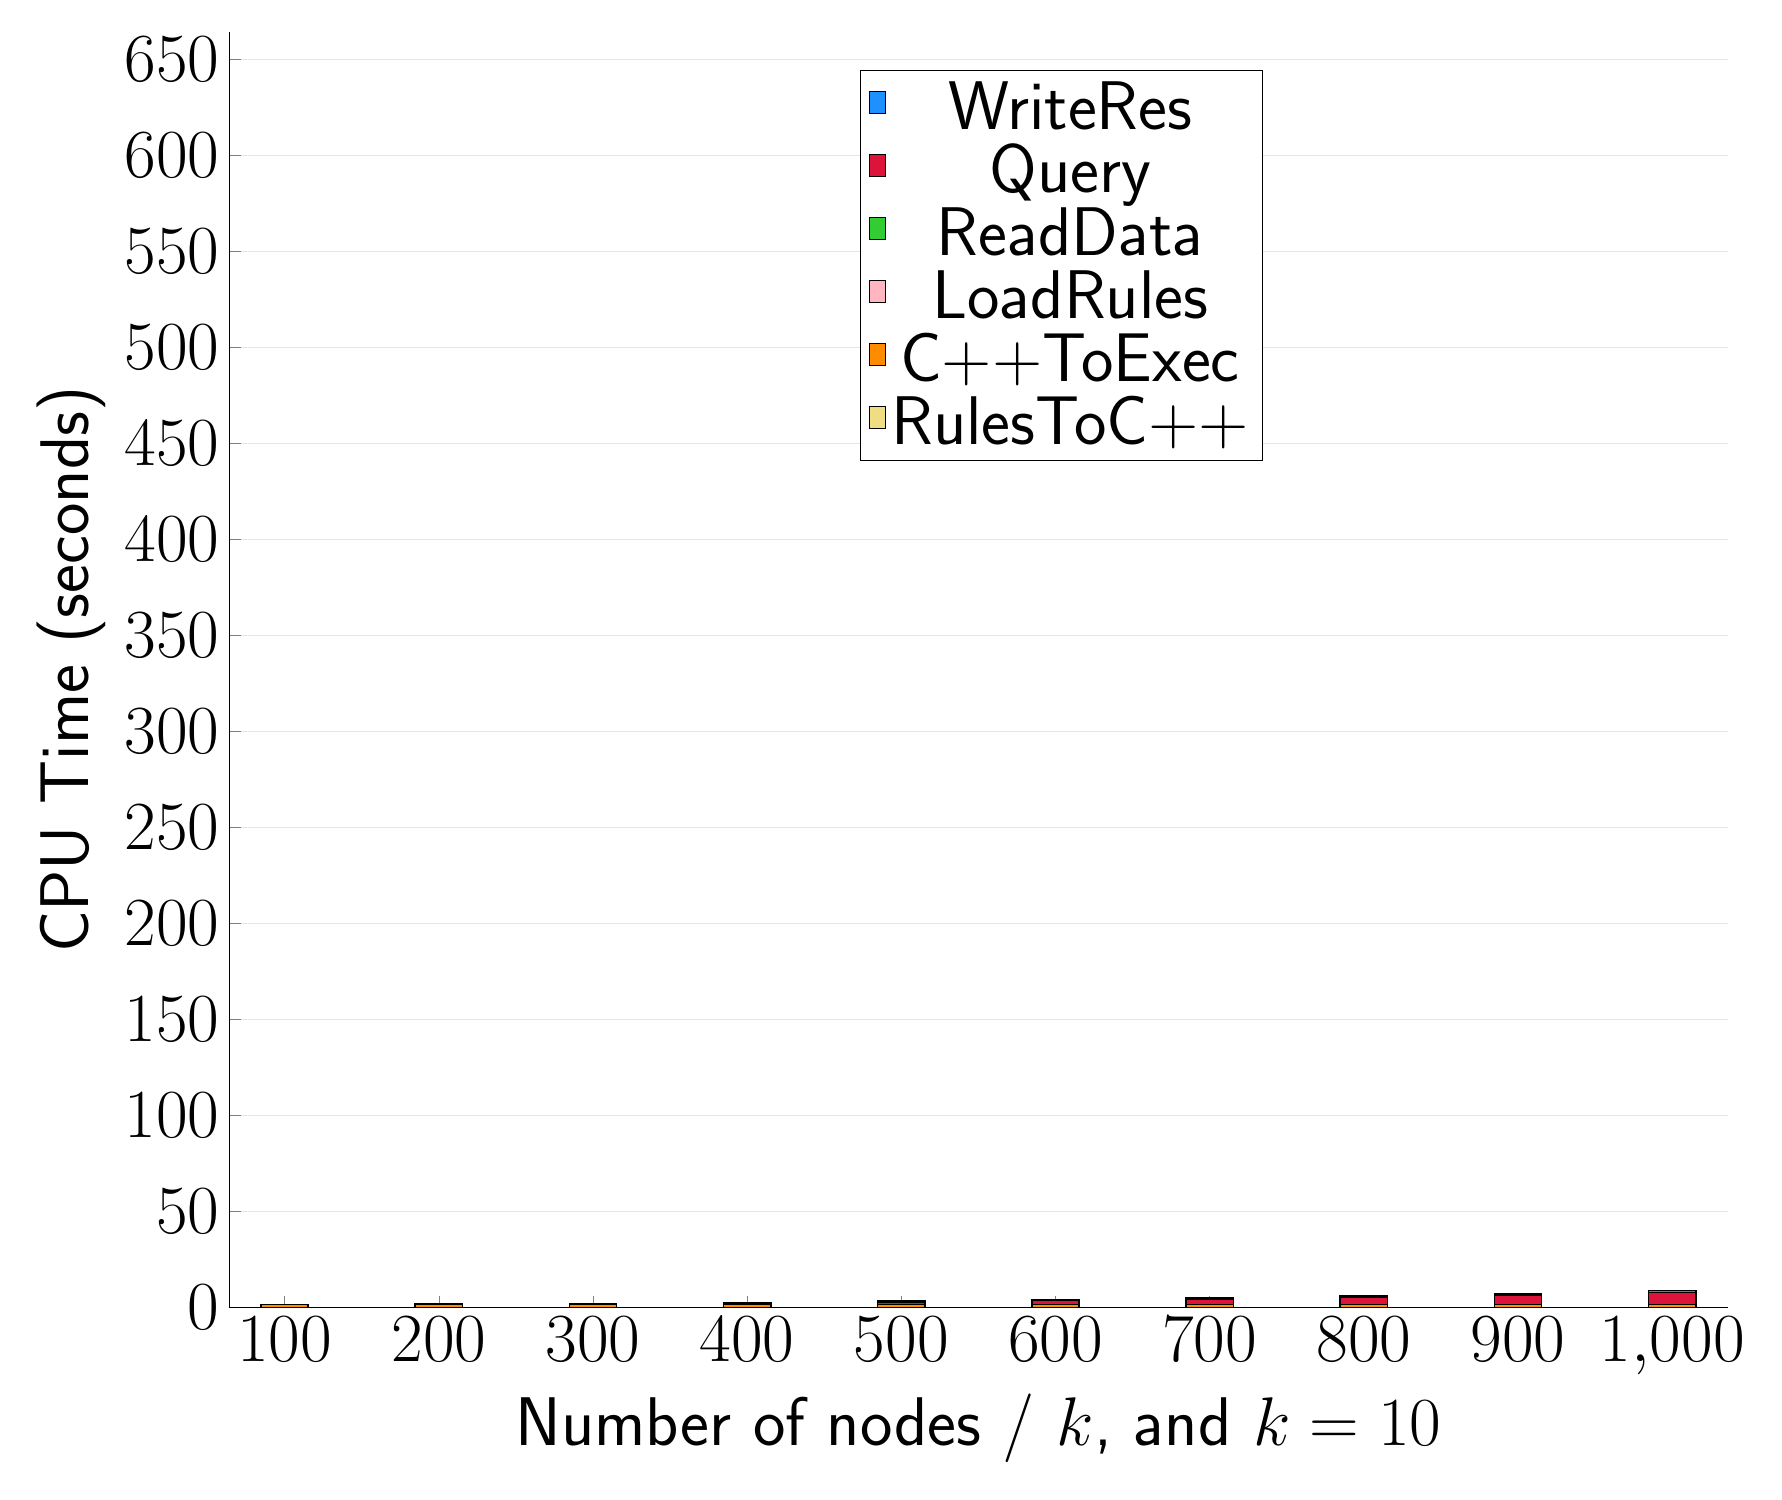
\begin{tikzpicture}
\begin{axis}[
   ybar stacked,
   width=1.7\textwidth,
   bar width=0.6cm,
   ymajorgrids, tick align=inside,
   major grid style={draw=gray!20},
   xtick=data,
   ymin=0, ymax=664.059,
   axis x line*=bottom,
   axis y line*=left,
   enlarge x limits=0.04,
   legend style={
       at={(0.69, 0.97)},
       anchor=north east,
       legend columns=1,
       font=\Huge,
   },
   ylabel={CPU Time (seconds)},
   xlabel={Number of nodes / $k$, and $k=10$},
   label style={font=\Huge},
   tick label style={font=\Huge},
]
\addlegendimage{fill=DodgerBlue, draw=black, line width=0.2pt}
\addlegendentry{WriteRes}
\addlegendimage{fill=Crimson, draw=black, line width=0.2pt}
\addlegendentry{Query}
\addlegendimage{fill=LimeGreen, draw=black, line width=0.2pt}
\addlegendentry{ReadData}
\addlegendimage{fill=LightPink, draw=black, line width=0.2pt}
\addlegendentry{LoadRules}
\addlegendimage{fill=DarkOrange, draw=black, line width=0.2pt}
\addlegendentry{C++ToExec}
\addlegendimage{fill=LightGoldenrod, draw=black, line width=0.2pt}
\addlegendentry{RulesToC++}
\addplot +[fill=LightGoldenrod, draw=black, line width=0.55pt] coordinates {
(100, 0.0020000000000000005)
(200, 0.004000000000000001)
(300, 0.006000000000000001)
(400, 0.0020000000000000005)
(500, 0.0020000000000000005)
(600, 0.006000000000000001)
(700, 0.006000000000000001)
(800, 0.0020000000000000005)
(900, 0.0020000000000000005)
(1000, 0.0020000000000000005)
};
\addplot +[fill=DarkOrange, draw=black, line width=0.55pt] coordinates {
(100, 1.4659999999999997)
(200, 1.472)
(300, 1.47)
(400, 1.4700000000000002)
(500, 1.472)
(600, 1.472)
(700, 1.474)
(800, 1.4780000000000002)
(900, 1.4740000000000002)
(1000, 1.4600000000000002)
};
\addplot +[fill=LightPink, draw=black, line width=0.55pt] coordinates {
(100, 0.0001648)
(200, 0.00016160000000000002)
(300, 0.0001718)
(400, 0.00017460000000000002)
(500, 0.00017839999999999997)
(600, 0.00016879999999999998)
(700, 0.0001764)
(800, 0.00015560000000000001)
(900, 0.00017859999999999998)
(1000, 0.0001346)
};
\addplot +[fill=LimeGreen, draw=black, line width=0.55pt] coordinates {
(100, 0.0040606)
(200, 0.007179200000000001)
(300, 0.010138999999999999)
(400, 0.013042199999999999)
(500, 0.0144368)
(600, 0.0176474)
(700, 0.0197192)
(800, 0.0186252)
(900, 0.0236118)
(1000, 0.021443999999999998)
};
\addplot +[fill=Crimson, draw=black, line width=0.55pt] coordinates {
(100, 0.0705446)
(200, 0.230699)
(300, 0.5187272)
(400, 0.9394866000000001)
(500, 1.486266)
(600, 2.15974)
(700, 2.9822819999999997)
(800, 3.9257280000000003)
(900, 5.0209600000000005)
(1000, 6.306964)
};
\addplot +[fill=DodgerBlue, draw=black, line width=0.55pt] coordinates {
(100, 0.010958199999999998)
(200, 0.0433486)
(300, 0.0969962)
(400, 0.17452120000000002)
(500, 0.2696992)
(600, 0.3851424)
(700, 0.525613)
(800, 0.7083472)
(900, 0.866398)
(1000, 1.079556)
};
\end{axis}
\end{tikzpicture}

\end{document}
